\def\tu{\vec\theta_{\uparrow}}
\def\td{\vec\theta_{\downarrow}}

\subsection{Linear Regression}

% TODO: Cite sources:
% - https://www.kaggle.com/c/house-prices-advanced-regression-techniques/data


% TODO: Sprinkle in actual examples from the data. Right now the explanation is highly theoretical, which is far from what we are trying to do (even though the concepts are purely theoretical...)

% TODO: Explain this better. It sounds robotic and unintuitive. This shit needs
% to be a STORY
The main focus of this section is predicting a real number when given a set of
other numbers, or using pre-recorded inputs and outputs to generate new outputs
for any input we may come across. In a linear sense, we are finding a continuous
function that takes in one number and spits out another using previously
gathered data. So the question is, how do we form this function?


Let's look at the scatterplot in Figure \ref{fig:hp}, which shows a bit of
housing data from Ames, Iowa. When observing it, our goal is to create a model
that will take a plot area and give us a house price that best fits the examples
recorded. So we start by asking, what kind of representation of data best aligns
with what we are asking? How can we find patterns in this data to predict what
price might be associated to a specified plot area? How can we do this
autonomously?

\begin{figure}[t!]
\centering
    \begin{tikzpicture}
        \selectcolormodel{gray}
        \begin{axis}[
                title = {HOUSE PRICES AND PLOT AREAS},  % whatever name you want
                xlabel = {Plot Area in 1,000 ft$^2$},
                ylabel = {House Price in \$100,000},
            ]
            \addplot[
                only marks,
                domain={4:18}
                ] table[col sep=comma]{linreg_houseprice.csv};
            \addplot[
            		gray,
            		thick,
            		dashed,
            		domain={4:18}
            ]{0.5 + 0.2*x};
            \addplot[
            		gray,
            		thick,
            		dotted,
            		domain={4:18}
            ]{0.1*x};
        \end{axis}
    \end{tikzpicture}
    \caption{List of plot areas and selling prices for houses in Ames, Iowa.
    Looking at these kind of plots, we can try to find correlations in the data
    that help us predict what future houses may cost in that market. The dashed line is our hypothesis with weights $\theta_{\uparrow}$ and the dotted line is our hypothesis with weights $\theta_{\downarrow}$.}
    \label{fig:hp}
\end{figure}

First, we can identify that there is a positive correlation when comparing each
plot area with its corresponding price, showing us that as plot area increases,
so does the house price. There are some outliers for this case, but generally
this trend is consistent. Additionally, we can take note that there is some
base price for every house in the area. Intuitively, we can
observe this by the fact that the goal of selling a house is to make money, so
assuming the smallest house you could buy is around 1,000 ft$^2$, we would
never see such a house costing \$0. As such, we should be able to draw a
straight line through the data from some offset such that we get fairly close
to all of the recorded examples.

This observation is the basis for any linear relationship of the form
$y=\theta_0 + \theta_1x$ with the bias $\theta_0$ describing the overall
starting price for houses in Ames and the correlation coefficient $\theta_1$
describing the correlation between housing price and plot area. When we assign
these variables as components to a vector $\vec\theta = \begin{pmatrix}\theta_0
\\ \theta_1\end{pmatrix}$, we end up with what's called the  \textbf{weight
vector} or just \textbf{weights}. With $\vec\theta$, we adjust the components
until we find coefficients that best model our data. 

Let $X$ be the training set, i.e. the set containing all of the
recorded plot areas. Let $X^{(i)}$ be the plot area for the $i$th feature in
$X$. From what we've discussed about the linear relationship, the equation
\begin{equation}
    hypothesis_{\vec\theta}(X^{(i)}) = \theta_0 + \theta_1X^{(i)}
\end{equation}
should hypothetically give us the correct price for $X^{(i)}$.

Now that we have a method of predicting values, it is helpful to see how
different choices of $\vec\theta$ interact with our hypothesis. Let us consider
two such choices:
\begin{equation*}
	\vec\theta_{\uparrow} = \begin{pmatrix}50000 \\ 200\end{pmatrix} \quad 	\vec\theta_{\downarrow} = \begin{pmatrix}0 \\ 100\end{pmatrix}
\end{equation*}
. The first choice $\vec\theta_{\uparrow}$ has a base price of \$50,000 and increases by \$200 per ft$^2$ of plot area. The second choice $\vec\theta_{\downarrow}$ has a base at \$0 and increases by \$100. As with all of science, we follow this scientific method of creating a hypothesis and testing its accuracy. If our hypothesis isn't accurate, we often reject it and look for a better estimation of our observations. This is no different for machine learning, so we first want to test this hypothesis to see how well it aligns with our observation. A meaningful question to then ask is: \emph{how well does our hypothesis predict values with these weights?}

For the first feature in our dataset with a plot area of 8,450 ft$^2$ we note the original price is \$208,500. When using weights $\vec\theta_{\uparrow}$ we will get the hypothetical price \$219,000 after calculation. Seems somewhat accurate, right? This price only overestimated the original by \$10,500 which is not terrible, specifically when compared to our hypothetical price  with weights $\vec\theta_{\downarrow}$, which gives us \$84,500 and underestimates the data by -\$124,000.

This measurement, the distance between our prediction and the recorded result,
is defined as the \textbf{loss} of our hypothesis. For the previous paragraph, we defined the loss as:
\begin{equation}\label{eq:incorrect loss}
	loss_{\vec\theta}(X^{(i)}) = hypothesis_{\vec\theta}(X^{(i)})-y^{(i)}
\end{equation}
. There is an issue with \ref{eq:incorrect loss} however, that being an inconsistent measurement between positive and negative values. Underestimations in the hypothesis, as we saw in $loss_{\vec\theta_{\downarrow}}(8450)$, result in a negative loss, which we can almost consider as a gain. This is flawed thinking since this is still an inaccuracy, and so should still be considered a loss. Considering this, we need a more consistant estimate for both overestimations and underestimations. The most apparent way of doing this would be taking the absolute value, making our loss function
\begin{equation}
	loss_{\vec\theta}(X^{(i)}) = |hypothesis_{\vec\theta}(X^{(i)}) - y^{(i)}|
\end{equation}
. This is a completely viable option. Another way of achieving this is by
squaring the loss
\begin{equation}
	loss_{\vec\theta}(X^{(i)}) = (hypothesis_{\vec\theta}(X^{(i)}) - y^{(i)})^2
\end{equation}
. Each of these have their own situational benefits discussed further in
\placeholder, however we will suffice to square the loss since its continuity
facilitates optimization as we shall see later in this section.

Now let's get back to the original question: how well does our hypothesis
predict values with these weights? Given what we have put together, it would
make sense to say our hypothesis performs well when our weights have a low
average loss across the data set since this would mean our average distance
between every prediction and recorded value is low. This measurement, the
effectiveness of our hypothesis using $\vec\theta$ across an entire data set, is
called the \textbf{cost} of $\vec\theta$. We then define the cost function as
\begin{subequations}
    \begin{align}
        cost(\vec\theta) = \avg_{1\leq i\leq m} (loss_{\vec\theta}(X^{(i)}, y^{(i)})) \\
    \intertext{or equivelently}
        cost(\vec\theta) = \frac{1}{m}\sum_{i=1}^m (\theta_0 + \theta_1X^{(i)} -
        y^{(i)})^2
    \end{align}
\end{subequations}
.

For our two choices of $\vec\theta$, we then have the costs
\begin{equation}\label{eq:tud cost results}
    cost(\vec\theta_{\uparrow})= \num{3.8e12} \quad \text{and} \quad
    cost(\vec\theta_{\downarrow}) = \num{7.4e11}
\end{equation}
. Our cost for $\td$ is lower than that of $\tu$, meaning that $\td$ generally
predicts values closer to our data set than $\tu$. Other then that, the
information this gives us is rather arbitrary. Since this is a squared distance,
this would mean the cost of $\td$ is $\num{7.4e11}$ squared dollars, an
absurdity considering the concept of a squared dollar is nonexistent in any
currency.  We could take the square root of the summation and find the average
amount of money that \emph{someone} is losing using weights $\td$ is about
\$120,719.73, providing us with a little more information on the matter.
However, this information does little for the computation and only serves to the
give humans contextual information, so the calculation is left out. This is
still an egregious sum to lose and surely we can find weights that minimize
this. Regardless, we now have an effective means of computing our weights'
performances in the hypothesis.

Since we now have a method of evaluating our hypothesis's performance with
weights $\vec\theta$, our next objective is to search for more suitable weights.
Continuing along the scientific method, the next question would be: \emph{how
can we adjust the hypothesis to better suit the data}, or in terms of what we've
covered, \emph{what are values of $\vec\theta$ that minimize this cost?}

We are looking for a base price and price per ft$^2$ that matches the data
enough such that the hypothesized price would be reasonably close to the
recorded price. What we're essentially looking for are the coordinates of a
point in the cost function's domain that correspond to the lowest lowest
possible value for the cost.
\begin{equation}
    \argmin_{\vec\theta} cost(\vec\theta) \Leftrightarrow \nabla
    cost(\vec\theta) = 0
\end{equation}
. To see how this is possible, let's consider the shape of the cost function.

The loss function expands out to be a second degree polynomial in two
dimensions, and we can identify each of the leading terms to be $\theta_0^2$ and
$\theta_1^2$. Because the dominating terms are all second degree, our domain and
range form an \emph{elliptical paraboloid} as seen in Figure \ref{fg:cost}. 

\begin{figure}[t!]
    \centering
    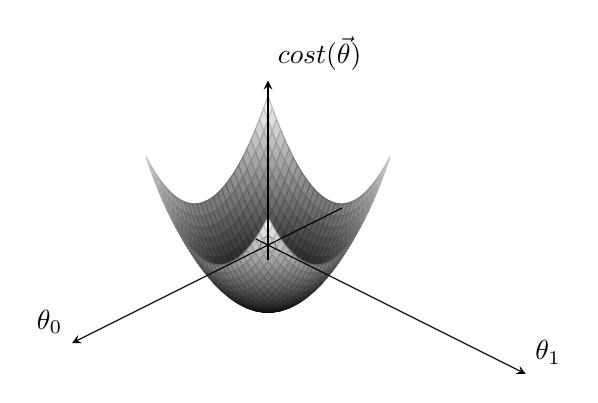
\begin{tikzpicture}[
        declare function = {
            Z(\x, \y) = ((\x-8)^2 + (\y-8)^2)/8;
        }
    ]
        \begin{axis}[
            view = {135}{30},
            colormap/blackwhite,
            axis equal,
            axis lines = center,
            axis on top,
            ticks = none,
            set layers = default
            xmin = 0, ymin = 0, zmin = 0,
            xlabel=$\theta_0$, ylabel={$\theta_1$}, zlabel={$cost(\vec\theta)$},
            xlabel style={anchor=south east},
            ylabel style={anchor=south west},
            zlabel style={anchor=south west},
            enlargelimits,
            tick align=inside,
            domain=0:16,
            y domain = 0:16,
            samples=30,
            z buffer=sort,
            minor tick=1,
            ]
            \addplot3 [surf] {Z(x, y)};
        \end{axis}
    \end{tikzpicture}
    \caption{The elliptical paraboloid formed by our weights $\vec\theta$ and $cost(\vec\theta)$.}
    \label{fg:cost}
\end{figure}

A direct consequence of this shape, as can be noted in the figure, is that a
global minimum is achievable since it is convex. As such, we can use
the methods described in Section \ref{st:gradient descent} about gradient
descent to find the coordinates that minimize the output of the cost function.
By doing this, we then find the optimal weights for our weight vector and
minimize the loss generated by the hypothesis.

 After the descent, we
end up with the weights converging to $\vec\theta_0 = \$71,663$ and
$\vec\theta_1 = \$10.79$ per ft$^2$ for both $\tu$ and $\td$. These are then the
minimal weights for the cost function, giving us the base price and price per
ft$^2$ that most accurately measure our data. As such, any new house price can
be estimated with a given plot area by:
\begin{equation}
    hypothesis_{\vec\theta}(X^{(i)}) = 71663 + 10.79X^{(i)}	
\end{equation}.
The cost of this these weights come out as $\num{4.1e9}$ which when using the
square root method discussed earlier comes out as an average loss of \$8,965.52
for any house in Ames, Iowa. This is a significant departure from the results
acheived in the results listed in Equation \ref{eq:tud cost results}, reducing our
average loss by over \$100,000.

% TODO: In Regularization/normalization, explain why inputs generally need to be scaled. This function with its weights already looks like
% \vec\theta_0^2 + \num{1e8}\vec\theta_1^2 + \num{2e4}\vec\theta_0\vec\theta_1 - \num{4e5}\vec\theta_0 - \num{4e9}\vec\theta_1 + \num{4e10}

% TODO: Discuss the following
%       - When should we dismiss the linear regression as an innacurate
%       measurement?

